\documentclass[11pt]{article}

\usepackage[margin=1in]{geometry}
\usepackage{microtype}
\usepackage{amsmath, amssymb}
\usepackage{booktabs}
\usepackage{enumitem}
\usepackage{xcolor}
\usepackage[round]{natbib}
\usepackage{hyperref}
\usepackage{tikz}
\usetikzlibrary{arrows.meta, positioning, fit, calc}
\hypersetup{
  colorlinks=true,
  linkcolor=black!70,
  citecolor=blue!50!black,
  urlcolor=blue!50!black,
}

\newcommand{\tok}[1]{\texttt{\small #1}}
\definecolor{pipeblue}{HTML}{2E5BFF}
\definecolor{pipebluefill}{HTML}{EEF3FF}
\definecolor{pipegreen}{HTML}{2E8B57}
\definecolor{pipegreenfill}{HTML}{EDF8F1}
\definecolor{pipegold}{HTML}{B7791F}
\definecolor{pipegoldfill}{HTML}{FFF8E8}
\definecolor{pipegrayfill}{HTML}{F3F4F6}
\definecolor{pipeink}{HTML}{2B2F38}

\title{\vspace{-1.1em}\textbf{Reasoning Motifs: A Tool for Understanding\\
Question-Local LLM Problem-Solving Patterns}\vspace{-0.5em}}

\author{%
  Author One\\\texttt{author1@student.ubc.ca}
  \and
  Author Two\\\texttt{author2@student.ubc.ca}
}
\date{}

\begin{document}
\maketitle
\thispagestyle{plain}
\renewcommand{\thefootnote}{}
\footnotetext{Course project for UBC CPSC 440/550, April 2026.}
\renewcommand{\thefootnote}{\arabic{footnote}}\setcounter{footnote}{0}

\begin{abstract}
\noindent We study whether \emph{question-local reasoning motifs} can be recovered from outcome-only supervision and used to organize mixed-outcome LLM trace pools. A local motif is a short typed subsequence mined within one math question and contrasted between correct and incorrect traces for that same question. The motivation is confound control: within-question comparisons hold the prompt fixed and therefore reduce the chance that question difficulty masquerades as reasoning quality. We evaluate the idea on one fixed dataset, \texttt{gpt\_oss\_subset\_15q\_all\_traces\_tokenized\_gpt-oss-chunked\_live\_1.csv}, containing 450 tokenized traces over 15 mixed-outcome questions. The main result is interpretive rather than leaderboard-oriented: local motif cards cover most questions and provide compact success/failure summaries for browsing traces. As a secondary sanity check, we run held-out-question prediction with logistic regression and compare motif features against raw-trace verbosity baselines computed from the original reasoning text. Under this stronger predictor, the best motif model reaches question-local AUC about 0.815: it remains below the raw-word baseline at 0.833, but is essentially tied with the raw-character baseline at 0.814. The resulting claim is still modest but more encouraging. Question-local motifs surface useful structural summaries and carry meaningful predictive signal, even though they are not yet clearly stronger than very simple raw-trace baselines.
\end{abstract}

\section{Introduction}

Reasoning models produce long chains of thought, yet the usual supervision signal is only whether the final answer is correct. Process supervision attacks this directly with step-level labels, but those labels are expensive to obtain at scale~\citep{lightman2023verify,wang2024mathshepherd}. Outcome-only supervision is much cheaper~\citep{deepseek-r1}, but it does not by itself reveal the recurring patterns a model uses while solving a problem.

Our project asks whether some process structure can still be extracted from outcome-only data in a form that helps a person inspect model behavior. We focus on \emph{question-local motifs}: typed bigrams or trigrams that recur within a single question and differ between successful and unsuccessful traces. The key reason to stay local is confounding. A pooled comparison across many questions can easily mistake difficulty for process. For example, certain algebraic operations may look ``good'' simply because they occur on easier questions, or ``bad'' simply because they occur on harder ones.

The contrastive intuition is simple. Suppose trace $i$ for question $q$ has outcome $Y_{qi}$ and feature vector $X_{qi}$, with
\begin{equation}
\Pr(Y_{qi}=1 \mid X_{qi}, q)=\sigma(\alpha_q + \beta^\top X_{qi}),
\label{eq:fixed-effect}
\end{equation}
where $\alpha_q$ is a question-specific difficulty term. In pooled analysis, $\alpha_q$ is a nuisance confounder. In a within-question comparison, however, $\alpha_q$ is shared across all traces of $q$ and therefore drops out of the local contrast. This does not make motif claims causal, but it gives a principled reason to prefer mixed-outcome, within-question analysis over global pooling.

The paper’s contribution is deliberately narrow. We do not claim to explain latent reasoning, and we do not present the project as an attempt to beat a predictive benchmark. Instead, we test whether a question-local motif representation is useful for understanding and organizing mixed-outcome trace pools on one fixed dataset. The answer is mixed but informative: the motif cards are interpretable and useful for browsing traces, while predictive checks suggest that the motif representation contains meaningful signal and can be competitive with simple raw-trace baselines, though not decisively better.

\paragraph{Contributions.}
\begin{enumerate}[leftmargin=*]
\item \textbf{Reasoning trace tokenization.} We build a typed tokenization scheme that rewrites free-form traces into \tok{action}, \tok{strategy}, \tok{milestone}, and \tok{noise} tokens suitable for downstream analysis.
\item \textbf{Sequence pattern mining.} We mine question-local contiguous bigrams and trigrams and compare them across correct and incorrect traces within the same problem.
\item \textbf{Motif-card interpretability tool.} We package the resulting local success/failure patterns into a small web app for understanding reasoning behavior and browsing mixed-outcome trace pools.
\item \textbf{Question-local evaluation framing.} We separate interpretability-first motif cards from a secondary predictive sanity check, and we evaluate the latter against raw-trace-only baselines rather than statistics derived from the tokenized representation itself.
\end{enumerate}

\section{Related Work}

The closest line of work is process supervision. \citet{lightman2023verify} show that step-level human labels can train strong verifiers, and \citet{wang2024mathshepherd} reduce the labeling burden by estimating step quality from rollout outcomes. Our setting is cheaper but weaker: we only assume final-answer correctness and try to recover inspectable local patterns rather than dense rewards.

A second relevant thread asks how trustworthy or informative chain-of-thought traces are. \citet{lanham2023faithfulness} and \citet{turpin2023unfaithful} show that externalized reasoning is not always a faithful report of hidden computation. We therefore treat motifs as behavioral summaries of emitted traces, not as guaranteed windows into the model’s internal algorithm. Finally, multi-trace reasoning methods such as self-consistency naturally create bags of traces per question~\citep{wang2023selfconsistency}; our project analyzes that trace pool rather than aggregating it away.

\section{Method}

All experiments in this paper use one frozen dataset:
\begin{center}
\tok{gpt\_oss\_subset\_15q\_all\_traces\_tokenized\_gpt-oss-chunked\_live\_1.csv}.
\end{center}
It contains 450 traces over 15 mixed-outcome math questions, with 297 correct traces and 153 incorrect traces. We do not evaluate the upstream rollout sampler here; we take this mixed-outcome subset as given and focus on the representation and analysis. Figure~\ref{fig:pipeline} summarizes the full project pipeline and highlights where the present paper is concentrated.

\begin{figure}[t]
\centering
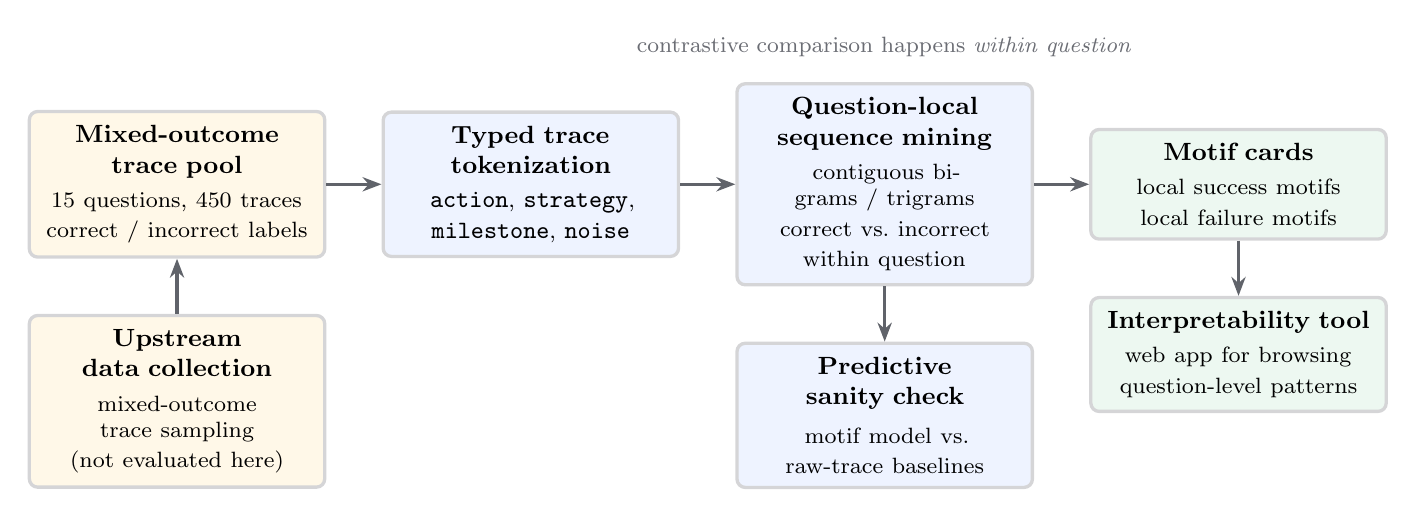
\begin{tikzpicture}[
  font=\small,
  node distance=7mm and 7mm,
  every node/.style={align=center},
  flow/.style={-{Stealth[length=2.4mm]}, very thick, draw=pipeink!75},
  box/.style={
    draw=pipeink!20,
    rounded corners=3pt,
    very thick,
    minimum height=11mm,
    text width=34mm,
    inner sep=5pt
  },
  inputbox/.style={box, fill=pipegoldfill},
  processbox/.style={box, fill=pipebluefill},
  outputbox/.style={box, fill=pipegreenfill},
  note/.style={font=\footnotesize, text=pipeink!70}
]

\node[inputbox] (data) {\textbf{Mixed-outcome trace pool}\\[1mm]
\footnotesize 15 questions, 450 traces\\
\footnotesize correct / incorrect labels};

\node[processbox, right=of data] (tok) {\textbf{Typed trace tokenization}\\[1mm]
\footnotesize \tok{action}, \tok{strategy},\\
\footnotesize \tok{milestone}, \tok{noise}};

\node[processbox, right=of tok] (mine) {\textbf{Question-local sequence mining}\\[1mm]
\footnotesize contiguous bigrams / trigrams\\
\footnotesize correct vs.\ incorrect within question};

\node[outputbox, right=of mine] (cards) {\textbf{Motif cards}\\[1mm]
\footnotesize local success motifs\\
\footnotesize local failure motifs};

\node[outputbox, below=of cards] (app) {\textbf{Interpretability tool}\\[1mm]
\footnotesize web app for browsing\\
\footnotesize question-level patterns};

\node[inputbox, below=of data] (sampling) {\textbf{Upstream data collection}\\[1mm]
\footnotesize mixed-outcome trace sampling\\
\footnotesize (not evaluated here)};

\node[processbox, below=of mine] (check) {\textbf{Predictive sanity check}\\[1mm]
\footnotesize motif model vs.\ raw-trace baselines};

\draw[flow] (data) -- (tok);
\draw[flow] (tok) -- (mine);
\draw[flow] (mine) -- (cards);
\draw[flow] (cards) -- (app);
\draw[flow] (mine) -- (check);
\draw[flow] (sampling) -- (data);

\node[note, above=2mm of mine] {contrastive comparison happens \emph{within question}};

\end{tikzpicture}
\caption{Project pipeline. Mixed-outcome trace collection happens upstream, but the present paper starts from a frozen trace set, tokenizes each reasoning trace, mines question-local sequence patterns, and packages them as motif cards for interpretability. Predictive performance is treated only as a secondary sanity check.}
\label{fig:pipeline}
\end{figure}

Each trace is already converted into a typed token sequence with tokens such as
\begin{center}
\tok{action:rewrite milestone:reduced-to-one-variable action:compute}.
\end{center}
The tokenization includes four token types: \tok{action}, \tok{strategy}, \tok{milestone}, and \tok{noise}. For motif mining, we keep only contiguous bigrams and trigrams, and we filter motifs containing answer-adjacent substrings such as \tok{final}, \tok{solution}, or \tok{answer}. This is meant to reduce leakage and keep the local summaries structurally meaningful.

Figure~\ref{fig:tokenizer-motif-pipeline} shows this transformation in the same visual language as the web app: a free-form reasoning trace is rewritten into typed token chips, contiguous token windows become candidate motifs, and repeated motifs are then surfaced as compact question-local cards.

\begin{figure}[t]
\centering
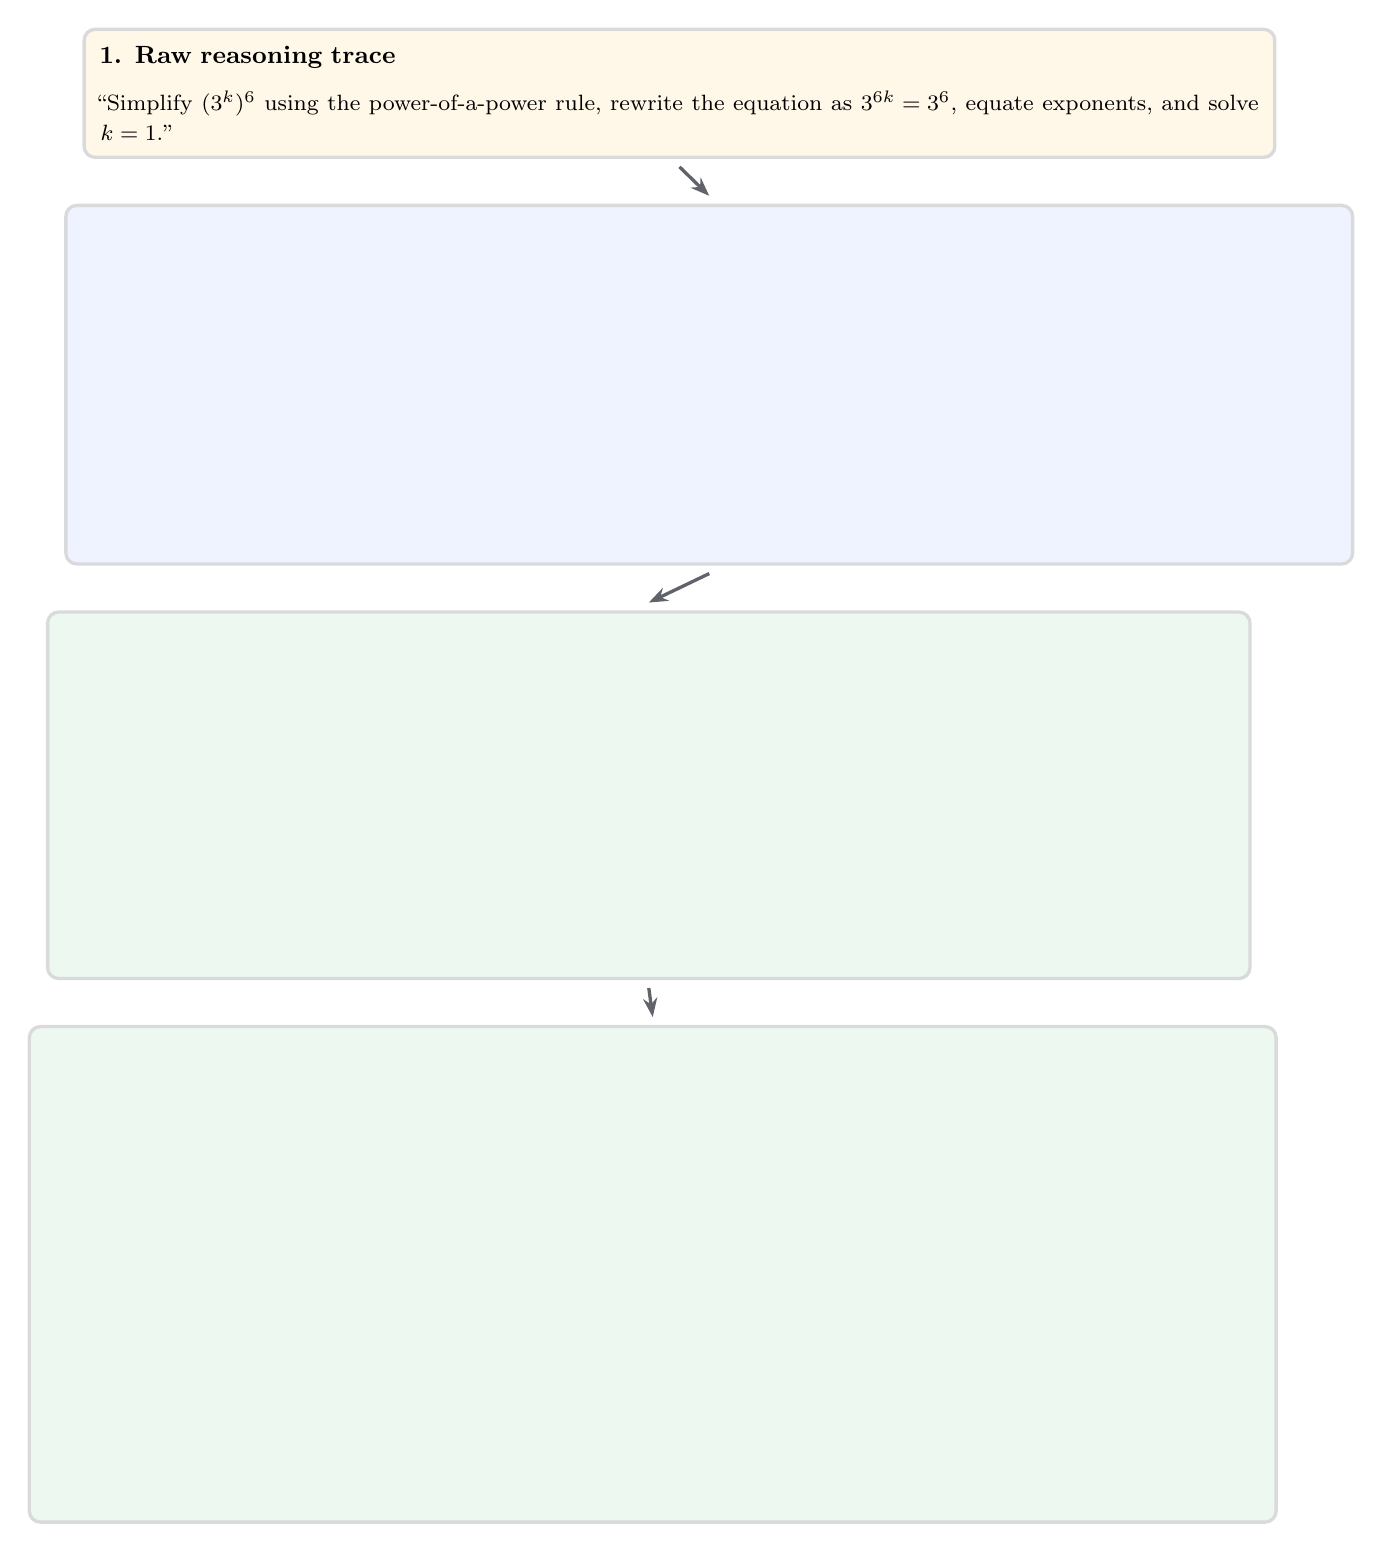
\begin{tikzpicture}[
  font=\small,
  panel/.style={
    draw=pipeink!18,
    rounded corners=4pt,
    very thick,
    inner sep=6pt
  },
  rawpanel/.style={panel, fill=pipegoldfill},
  tokenpanel/.style={panel, fill=pipebluefill},
  motifpanel/.style={panel, fill=pipegreenfill},
  chip/.style={
    draw=pipeink!18,
    rounded corners=9pt,
    inner xsep=4pt,
    inner ysep=2.5pt,
    font=\scriptsize\ttfamily
  },
  actionchip/.style={chip, fill=pipebluefill},
  strategychip/.style={chip, fill=pipegoldfill},
  milestonechip/.style={chip, fill=pipegreenfill},
  noisechip/.style={chip, fill=pipegrayfill},
  stage/.style={font=\small\bfseries, text=pipeink},
  note/.style={font=\footnotesize, text=pipeink!75},
  flow/.style={-{Stealth[length=2.4mm]}, very thick, draw=pipeink!75}
]

\node[rawpanel, text width=14.7cm, anchor=north west] (raw) at (0,0) {%
\textbf{1. Raw reasoning trace}\par
\medskip
\footnotesize
``Simplify $(3^k)^6$ using the power-of-a-power rule, rewrite the equation as
$3^{6k}=3^6$, equate exponents, and solve $k=1$.''};

\node[stage, anchor=north west] (toktitle) at ([xshift=0mm,yshift=-8mm]raw.south west)
{2. Typed tokenizer rewrites free-form spans into canonical labels};

\node[actionchip, anchor=north west] (t1) at ([xshift=4mm,yshift=-7mm]toktitle.south west) {action:apply-formula};
\node[milestonechip, right=2mm of t1] (t2) {milestone:applied:power-of-a-power};
\node[actionchip, right=2mm of t2] (t3) {action:compare};

\node[milestonechip, anchor=north west] (t4) at ([xshift=4mm,yshift=-4mm]t1.south west) {milestone:equation-simplified};
\node[strategychip, right=2mm of t4] (t5) {strategy:equate-exponents};
\node[actionchip, right=2mm of t5] (t6) {action:derive-intermediate};

\node[milestonechip, anchor=north west] (t7) at ([xshift=4mm,yshift=-4mm]t4.south west) {milestone:key-relation:exponents-equal};
\node[strategychip, right=2mm of t7] (t8) {strategy:solve-linear};
\node[actionchip, right=2mm of t8] (t9) {action:compute};
\node[milestonechip, right=2mm of t9] (t10) {milestone:derived:solution};

\node[actionchip, anchor=north west] (l1) at ([xshift=4mm,yshift=-5mm]t7.south west) {action};
\node[strategychip, right=2mm of l1] (l2) {strategy};
\node[milestonechip, right=2mm of l2] (l3) {milestone};
\node[noisechip, right=2mm of l3] (l4) {noise};
\node[note, right=3mm of l4] (legend) {token families used by the tokenizer};

\node[tokenpanel, fit=(toktitle)(t1)(t2)(t3)(t4)(t5)(t6)(t7)(t8)(t9)(t10)(l1)(legend)] (tokpanel) {};

\node[stage, anchor=north west] (motiftitle) at ([xshift=0mm,yshift=-8mm]tokpanel.south west)
{3. Contiguous token windows become candidate motifs};
\node[note, anchor=north west, text width=14.2cm] (motifnote) at ([xshift=4mm,yshift=-4mm]motiftitle.south west)
{Enumerate all contiguous 1-, 2-, and 3-token subsequences. For prediction we
deduplicate within a trace, so a motif counts at most once per document.};

\node[strategychip, anchor=north west] (m1a) at ([xshift=8mm,yshift=-5mm]motifnote.south west) {strategy:equate-exponents};
\node[actionchip, right=2mm of m1a] (m1b) {action:derive-intermediate};
\node[milestonechip, right=2mm of m1b] (m1c) {milestone:key-relation:exponents-equal};

\node[strategychip, anchor=north west] (m2a) at ([xshift=8mm,yshift=-4mm]m1a.south west) {strategy:solve-linear};
\node[actionchip, right=2mm of m2a] (m2b) {action:compute};
\node[milestonechip, right=2mm of m2b] (m2c) {milestone:derived:solution};

\node[actionchip, anchor=north west] (m3a) at ([xshift=8mm,yshift=-4mm]m2a.south west) {action:compare};
\node[milestonechip, right=2mm of m3a] (m3b) {milestone:equation-simplified};

\node[motifpanel, fit=(motiftitle)(motifnote)(m1a)(m1b)(m1c)(m2a)(m2b)(m2c)(m3a)(m3b)] (motifpanelbox) {};

\node[stage, anchor=north west] (cardtitle) at ([xshift=0mm,yshift=-8mm]motifpanelbox.south west)
{4. Question-local motif cards summarize repeated, high-contrast patterns};
\node[note, anchor=north west, text width=14.2cm] (cardnote) at ([xshift=4mm,yshift=-4mm]cardtitle.south west)
{Across all traces for the same question $q$, motif support is compared between
correct and incorrect traces. The web app then displays the strongest motifs as
compact chips.};

\node[panel, fill=white, text width=6.5cm, anchor=north west] (cardbox) at ([xshift=8mm,yshift=-6mm]cardnote.south west) {%
\textbf{Example motif card}\par
\medskip
\scriptsize Success-leaning motifs\par
\medskip
\tok{strategy:solve-linear | action:compute}\par
\tok{action:compute | milestone:derived:solution}\par
\tok{action:compare | milestone:equation-simplified}\par
\medskip
\footnotesize $\Delta_q(m)=\Pr(m\mid \text{correct},q)-\Pr(m\mid \text{incorrect},q)$};

\node[note, anchor=north west, text width=6.2cm] (cardside) at ([xshift=8mm]cardbox.north east)
{This mirrors the webapp view: rounded chips provide a compact visual summary,
while clicking through reveals the full tokenized trace and raw reasoning trace
that produced each motif.};

\node[motifpanel, fit=(cardtitle)(cardnote)(cardbox)(cardside)] (cardpanel) {};

\draw[flow] ([xshift=0mm,yshift=-1mm]raw.south) -- ([yshift=1mm]tokpanel.north);
\draw[flow] ([xshift=0mm,yshift=-1mm]tokpanel.south) -- ([yshift=1mm]motifpanelbox.north);
\draw[flow] ([xshift=0mm,yshift=-1mm]motifpanelbox.south) -- ([yshift=1mm]cardpanel.north);

\end{tikzpicture}
\caption{Tokenizer-to-motif pipeline drawn natively in LaTeX/TikZ and styled after the motif webapp. A free-form reasoning trace is first rewritten into typed token families, then expanded into contiguous token motifs, and finally aggregated into compact question-local motif cards.}
\label{fig:tokenizer-motif-pipeline}
\end{figure}

For any motif feature $X$, the basic local quantity is
\begin{equation}
\Delta_q(X)=\mathbb{E}[X \mid \text{correct}, q]-\mathbb{E}[X \mid \text{incorrect}, q],
\label{eq:delta}
\end{equation}
so the unit of analysis is the question rather than the pooled corpus.

From this representation we build \emph{motif cards}. Each question gets a small set of success-enriched motifs and failure-enriched motifs, ranked by local evidence subject to a minimum support threshold of 2. Sequence pattern mining is deliberately simple: motifs are contiguous subsequences of length 2 or 3, so the representation stays interpretable and the combinatorics stay manageable on a small course-project dataset. We then run two analyses:
\begin{enumerate}[leftmargin=*]
\item \textbf{Coverage / inspection analysis.} Do motif cards cover enough of the trace pool to be a useful browsing tool?
\item \textbf{Predictive sanity check.} How much predictive signal do the same motifs carry relative to simple baselines defined only on the original raw reasoning trace?
\end{enumerate}

\section{Experiments and Analysis}

\subsection{Dataset summary}

The dataset is moderately sized but still small enough that sparsity matters. The average tokenized trace length is 11.96 tokens, and 21.6\% of traces contain at least one \tok{noise:corrupted-span} token. After filtering to local bigrams and trigrams, the surfaced motif-card inventory covers 283 of 450 traces (62.9\%) and 14 of 15 questions (93.3\%).

\begin{table}[h]
\centering
\small
\caption{Summary of the fixed 15-question dataset used for all experiments.}
\label{tab:dataset}
\begin{tabular}{@{}lr@{}}
\toprule
Statistic & Value \\
\midrule
Questions & 15 \\
Traces & 450 \\
Correct / incorrect & 297 / 153 \\
Average tokenized length & 11.96 \\
Traces with noise token & 21.6\% \\
Trace coverage by surfaced motifs & 62.9\% \\
Question coverage by surfaced motifs & 93.3\% \\
\bottomrule
\end{tabular}
\end{table}

\subsection{Experiment 1: are motif cards useful summaries?}

This first analysis asks whether the local motif cards produce readable summaries of a mixed-outcome trace pool. The answer is yes, at least qualitatively. Many questions surface distinct success and failure motifs that are easier to inspect than dozens of raw chains of thought. These cards are exposed in a lightweight web app whose purpose is interpretability rather than prediction: it lets a user browse a question, inspect its local success and failure motifs, and drill into the corresponding traces. Table~\ref{tab:examples} shows three representative examples from the current explorer.

\begin{table}[h]
\centering
\small
\caption{Example local motifs surfaced by the motif-card pipeline.}
\label{tab:examples}
\begin{tabular}{@{}p{8mm}p{45mm}p{45mm}@{}}
\toprule
QID & Success motifs & Failure motifs \\
\midrule
45 & \tok{action:apply-formula action:rewrite}; \tok{action:compute milestone:derived:closed-form} & \tok{action:analyze strategy:set-subgoal} \\
52 & \tok{action:compute milestone:key-relation:numerator-simplified}; \tok{action:compute milestone:key-relation:denominator-simplified} & \tok{strategy:choose-representation action:compute} \\
68 & \tok{action:apply-formula action:derive-intermediate action:rewrite}; \tok{action:compare action:conclude} & \tok{action:analyze action:instantiate action:rewrite}; \tok{action:rewrite strategy:set-subgoal} \\
\bottomrule
\end{tabular}
\end{table}

These examples support a modest positive claim: the representation is structured enough to surface question-specific differences between successful and unsuccessful traces. This makes motif cards useful as a browsing or triage layer, even before asking whether they are strong predictors.

\subsection{Experiment 2: predictive power of motifs against raw-trace baselines}

The second analysis asks whether the same local motif representation carries predictive signal under a question-holdout evaluation. We use 5-fold cross-validation over questions: all traces from a held-out question are excluded from training, and the model must rank correct and incorrect traces for entirely unseen prompts. Both the motif model and the scalar baselines are fit with logistic regression so that the comparison is model-matched: motif prediction uses a sparse logistic regression over motif presence, while the raw-trace baselines use one-dimensional logistic regression over length. This predictive experiment is distinct from the question-local card construction itself: the model operates on a shared motif vocabulary induced by the typed tokenization, not by mining a fresh motif card directly from the held-out question. We report both global AUC and question-local AUC, where the latter averages within-question rankings and is the more relevant metric for our contrastive setting.

To avoid treating tokenized-trace statistics as an external baseline, we compare motifs only against \emph{raw-trace} baselines computed from the original \texttt{reasoning\_trace} field before tokenization. We consider two such baselines: raw word count and raw character count. Both use no motif identity and no information derived from the tokenized representation itself. Because the scalar baseline is also trained with logistic regression, it automatically learns whether longer or shorter traces should correspond to higher correctness on the training folds.

We also vary the motif support threshold. Interpreting ``support $>2$'' and ``support $>3$'' literally, we evaluate minimum support thresholds of 3 and 4, alongside a stricter threshold of 12. Table~\ref{tab:predictive} shows the resulting question-local comparison.

\begin{table}[h]
\centering
\small
\caption{Question-local predictive performance on the fixed 15-question dataset. Deltas are motif Q-local AUC minus the corresponding raw-trace baseline after learning baseline direction on the training folds.}
\label{tab:predictive}
\begin{tabular}{@{}lccccc@{}}
\toprule
Support rule & Motif Q-local AUC & Raw-word baseline & $\Delta$ vs.\ words & Raw-char baseline & $\Delta$ vs.\ chars \\
\midrule
\texttt{support $\geq 3$}  & 0.815 & 0.833 & -0.018 & 0.814 & +0.001 \\
\texttt{support $\geq 4$}  & 0.809 & 0.833 & -0.024 & 0.814 & -0.004 \\
\texttt{support $\geq 12$} & 0.813 & 0.833 & -0.020 & 0.814 & -0.001 \\
\bottomrule
\end{tabular}
\end{table}

Under this logistic-regression evaluation, motifs carry meaningful predictive signal and come much closer to the raw-trace baselines than in the earlier Naive Bayes version of the experiment. The best motif configuration here is actually the more permissive support threshold of 3, which reaches question-local AUC 0.815. Support thresholds of 4 and 12 remain close behind at 0.809 and 0.813. This suggests that once the classifier can combine many motifs discriminatively, lower-support features are less damaging than they were under the earlier model.

The raw baselines are still strong. Raw word count reaches question-local AUC 0.833, while raw character count reaches 0.814. The best motif model therefore still trails the raw-word baseline by a small margin, but is effectively tied with the raw-character baseline. This is a more nuanced and more encouraging result than the earlier draft: simple raw-trace verbosity remains a strong signal, but a sparse motif model can recover nearly the same within-question ranking performance while providing a far more interpretable representation.

This updated result supports a balanced claim. We still do not present local motifs as the strongest available correctness predictor on this dataset. However, under a stronger model that combines many motifs jointly, the motif representation is no longer obviously dominated by raw-trace baselines. The main value of the representation remains interpretive, but the predictive sanity check is now more supportive: local motifs appear to capture a substantial fraction of the same question-local ranking signal while also exposing which structural patterns drive the score.

\section{Discussion and Future Work}

The main strength of the project is conceptual and practical. The contrastive, question-local framing is a principled way to reduce difficulty confounding when only outcome labels are available, and the resulting motif-card interface gives a usable way to inspect patterns in a bag of reasoning traces.

The main weakness is still empirical. On this dataset, local motifs are not yet a clearly dominant predictive explanation layer. They cover many questions and look meaningful to a human reader, and under logistic regression they become competitive with raw-trace length baselines, but they still do not cleanly surpass the strongest of those baselines. That forces a narrower and more honest claim: local motifs are currently best justified as a tool for understanding and inspecting reasoning behavior, with predictive usefulness as a secondary benefit rather than the central result.

There are at least three reasons the method may be underperforming:
\begin{enumerate}[leftmargin=*]
\item \textbf{The dataset is small and heterogeneous.} Even within one question, there can be several successful reasoning paths and several distinct failure patterns.
\item \textbf{The tokenization is lossy.} Similar strategic moves may appear under different local surface forms, fragmenting support across motifs.
\item \textbf{Outcome-only labels are noisy process proxies.} Final correctness is relevant, but it is still a weak supervision signal for local reasoning quality.
\end{enumerate}

With more time, we would push in two directions. First, we would evaluate motif cards as a human-facing analysis tool: do they actually help someone inspect mixed-outcome trace pools faster or better than raw traces alone? Second, we would test richer local tokenizations that preserve strategic structure while reducing sparsity, since the current failure may reflect the representation more than the contrastive idea itself.

\section*{Acknowledgments}

We thank the course staff for the project framing and feedback.

\begin{thebibliography}{10}

\bibitem[DeepSeek-AI(2025)]{deepseek-r1}
DeepSeek-AI.
\newblock DeepSeek-R1: Incentivizing Reasoning Capability in Language Models via Reinforcement Learning.
\newblock \emph{arXiv:2501.12948}, 2025.

\bibitem[Lanham et~al.(2023)]{lanham2023faithfulness}
T.~Lanham, A.~Chen, A.~Radhakrishnan, et al.
\newblock Measuring Faithfulness in Chain-of-Thought Reasoning.
\newblock \emph{Anthropic Technical Report}, 2023.

\bibitem[Lightman et~al.(2023)]{lightman2023verify}
H.~Lightman, V.~Kosaraju, Y.~Burda, et al.
\newblock Let's Verify Step by Step.
\newblock \emph{arXiv:2305.20050}, 2023.

\bibitem[Turpin et~al.(2023)]{turpin2023unfaithful}
M.~Turpin, J.~Michael, E.~Perez, S.~R.~Bowman.
\newblock Language Models Don't Always Say What They Think: Unfaithful Explanations in Chain-of-Thought Prompting.
\newblock \emph{NeurIPS}, 2023.

\bibitem[Wang et~al.(2023)]{wang2023selfconsistency}
X.~Wang, J.~Wei, D.~Schuurmans, Q.~Le, E.~Chi, S.~Narang, A.~Chowdhery, D.~Zhou.
\newblock Self-Consistency Improves Chain of Thought Reasoning in Language Models.
\newblock \emph{ICLR}, 2023.

\bibitem[Wang et~al.(2024)]{wang2024mathshepherd}
P.~Wang, L.~Li, Z.~Shao, R.~X.~Xu, D.~Dai, Y.~Li, D.~Chen, Y.~Wu, Z.~Sui.
\newblock Math-Shepherd: Verify and Reinforce LLMs Step-by-Step Without Human Annotations.
\newblock \emph{ACL}, 2024.

\end{thebibliography}

\end{document}
